%% LyX 2.0.6 created this file.  For more info, see http://www.lyx.org/.
%% Do not edit unless you really know what you are doing.
\documentclass[spanish]{article}
\usepackage[T1]{fontenc}
\usepackage[utf8]{luainputenc}
\usepackage{geometry}
\geometry{verbose,tmargin=2cm,bmargin=2cm,lmargin=2cm,rmargin=2cm}
\usepackage{graphicx}

\makeatletter

%%%%%%%%%%%%%%%%%%%%%%%%%%%%%% LyX specific LaTeX commands.
%% Because html converters don't know tabularnewline
\providecommand{\tabularnewline}{\\}

%%%%%%%%%%%%%%%%%%%%%%%%%%%%%% User specified LaTeX commands.
\usepackage{multicol}
\usepackage{enumitem}
\date{}

\makeatother

\usepackage[english]{babel}
\addto\shorthandsspanish{\spanishdeactivate{~<>.}}

\begin{document}

\section{Que es un Grafo?}

Dicho formalmente un Grafo es un conjunto de Vértices y Arcos.

\[
G=\{V,A\}
\]


Pero un Vértice puede representar cualquier cosa (ciudades, personas,
objetos, etc) y los Arcos son las relaciones que tienen esos Vértices,
desde este punto de vista un Grafo puede representar cualquier cosa
que queramos (para los entusiastas la vida es un Grafo).

\begin{multicols}{2}

\begin{center}

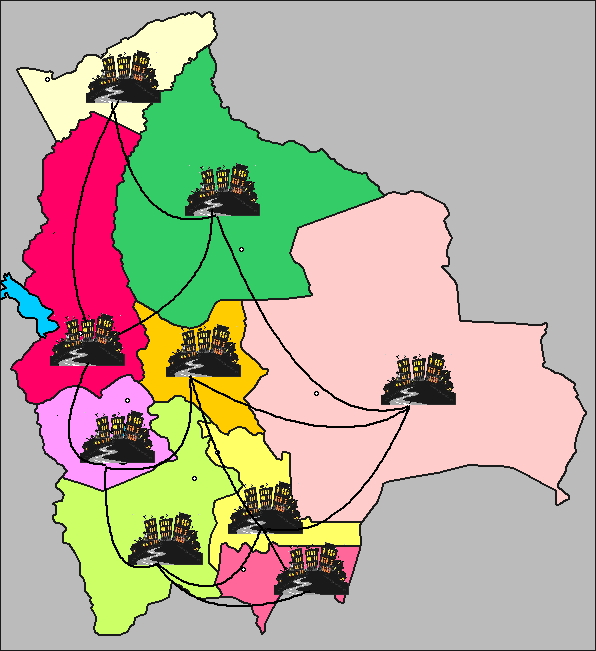
\includegraphics[scale=0.3]{Ej_Mapa}

Figura 1:Grafo donde las ciudades son Vértices y las carreteras los
Arcos.

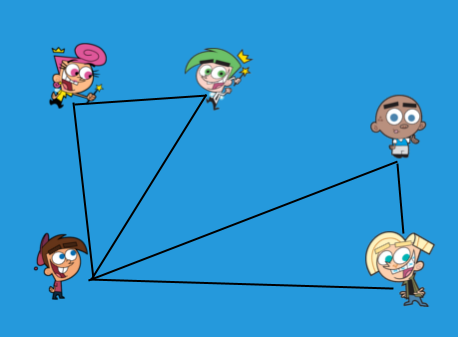
\includegraphics[scale=0.6]{Ej-Amistad}

Figura 2:Grafo donde las personas son Vértices y los Arcos representan
amistad.

\end{center}

\end{multicols}

Teniendo en cuenta esto nos podemos dar cuenta que desde que nos levantamos
estamos modelando grafos, estamos recorriendo grafos.

Ejemplo 1.

Una persona que se encuentre en el Stadium y quiera llegar al Aeropuerto,
su cerebro inconcientemente ya esta modelando un grafo donde tenemos
los lugares(Vertices) y las calles que nos llevan a ellos (Arcos):

\begin{center}

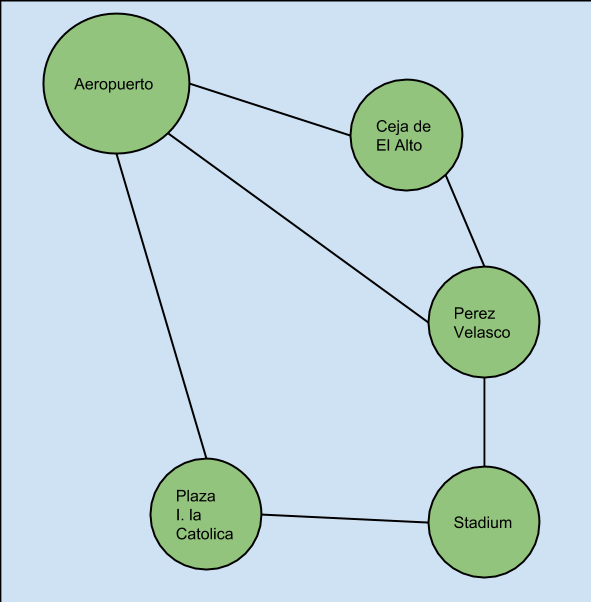
\includegraphics[scale=0.4]{Ejemplo_Grafo_01}

\end{center}

Ahora podemos ver los posibles caminos que nos llevan desde el Stadium
hasta el Aeropuerto, pero ?que pasa si queremos saber por que camino
gasto menos dinero o por cual llego mas rápido?

\begin{multicols}{2}

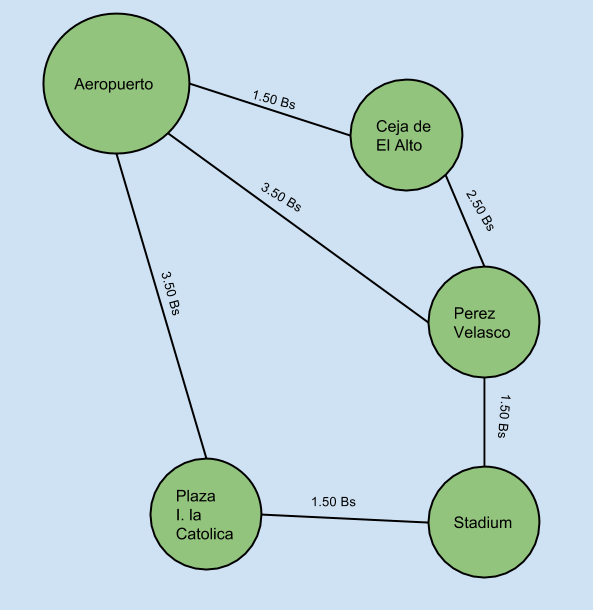
\includegraphics[scale=0.4]{Ejemplo_Grafo_02} 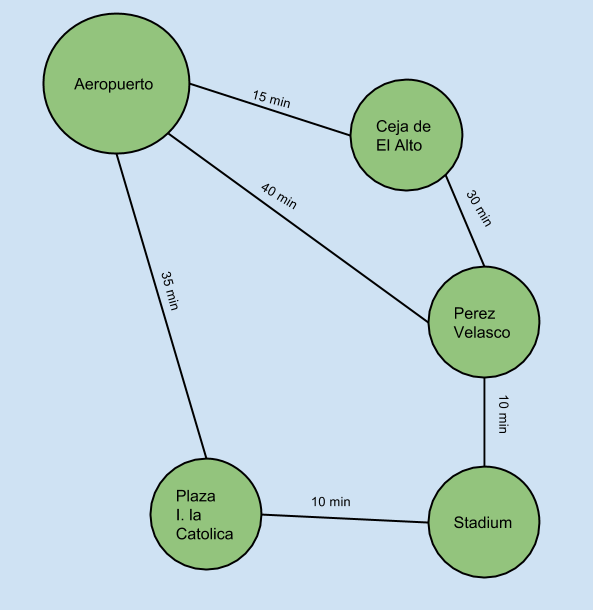
\includegraphics[scale=0.4]{Ejemplo_Grafo_03}

\end{multicols}

Cuando a los arcos se le da un valor se llama, Grafo Ponderado. Ahora,
si es que nosotros vamos en nuestro propio automovil seria bueno saber
que caminos podemos tomar:

\begin{center}

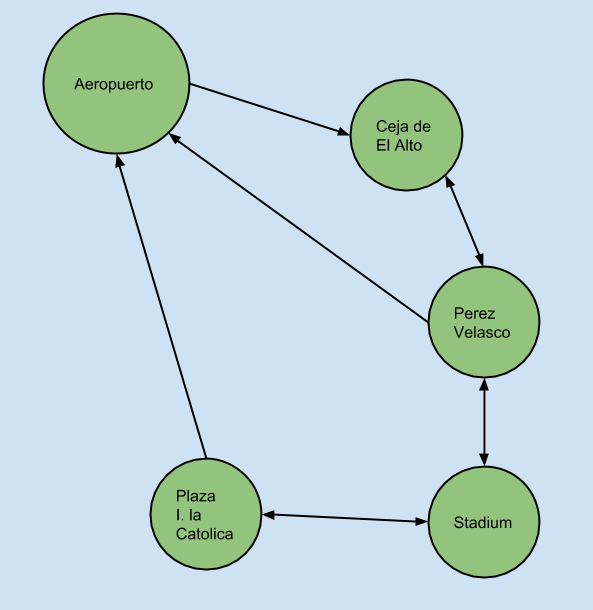
\includegraphics[scale=0.4]{Ejemplo_Grafo_04}

\end{center}

Cuando el grafo tiene caminos que solo se pueden usar de un sentido,Ej.
Perez Velasco-Aeropuerto, se le llama Grafo Dirigido.

Como podemos ver tenemos 4 tipos de grafos:
\begin{itemize}
\item Grafo dirigido-ponderado
\item Grafo no dirigido-no ponderado
\item Grafo dirigido-no ponderado
\item Grafo no dirigido-ponderado
\end{itemize}
Entonces como vimos con grafos podemos representar muchísimas cosas
de la vida diaria, es por esto que en las Ciencias de la Computación
un Grafo es usado como una Estructura de Datos, en concreto un tipo
de Dato Abstracto, es decir un conjunto de datos sobre los que podemos
hacer operaciones definas. Muchos problemas, especialmente de las
Olimpiadas y Competencias, tiene su solución con el uso de los grafos. 

En este punto en el que ya sabemos que es un grafo, tenemos la idea
de como modelarlos, surge la duda ?Como puedo representar un grafo
al momento de programar?


\section{Representacion de un grafo}

Con todo lo aprendido estamos listos, para representar el grafo, para
esto usaremos las 2 formas mas comunes de represnetar un grafo:


\subsection{Matriz de Adyacencia}

La forma mas fácil (pero no la mas eficiente) de representar un grafo
es usando una Matriz, como podemos ver a continuación:

\begin{center}

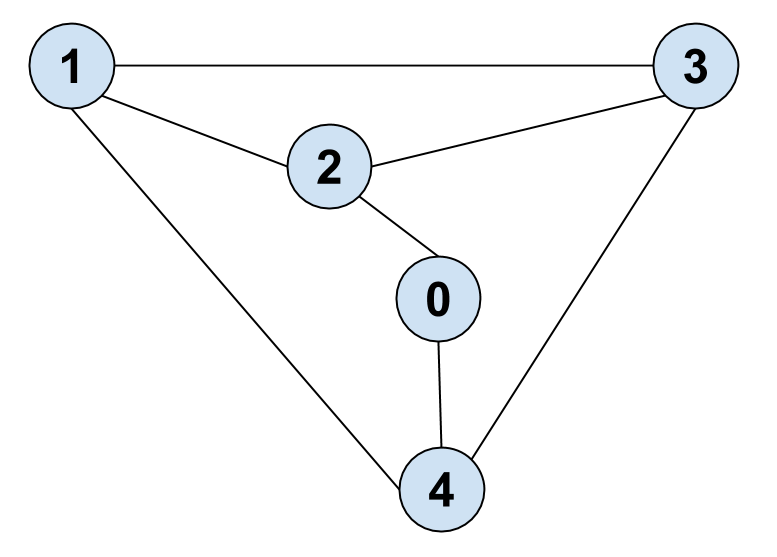
\includegraphics[scale=0.2]{Grafo_01} %
\begin{tabular}{|c|c|c|c|c|c|}
\hline 
I\textbackslash{}J & 0 & 1 & 2 & 3 & 4\tabularnewline
\hline 
\hline 
0 & 0 & 0 & 1 & 0 & 1\tabularnewline
\hline 
1 & 0 & 0 & 1 & 1 & 1\tabularnewline
\hline 
2 & 1 & 1 & 0 & 1 & 0\tabularnewline
\hline 
3 & 0 & 1 & 1 & 0 & 1\tabularnewline
\hline 
4 & 1 & 1 & 0 & 1 & 0\tabularnewline
\hline 
\end{tabular}\end{center}

Si es un grafo sin pesos, podemos usar una Matriz booleana donde marcamos
'1' o ``true'' si es que existe un arco del vértice 'i' al vértice
'j' y colocamos '0' o ``false'' en el caso que no haya un arco entre
esos vértices, acá tenemos el código general para representar un grafo
como Matriz de Adyacencia:

\begin{center}

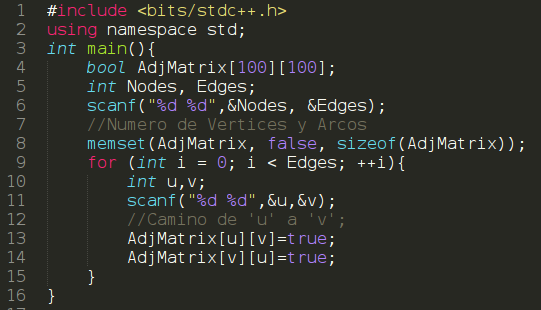
\includegraphics[scale=0.4]{Codigo_Grafo_01}

\end{center}

Si los arcos tienen pesos, es decir si es ponderado, lo colocamos
en la casilla (i,j), como se muestra a continuación:

\begin{center}

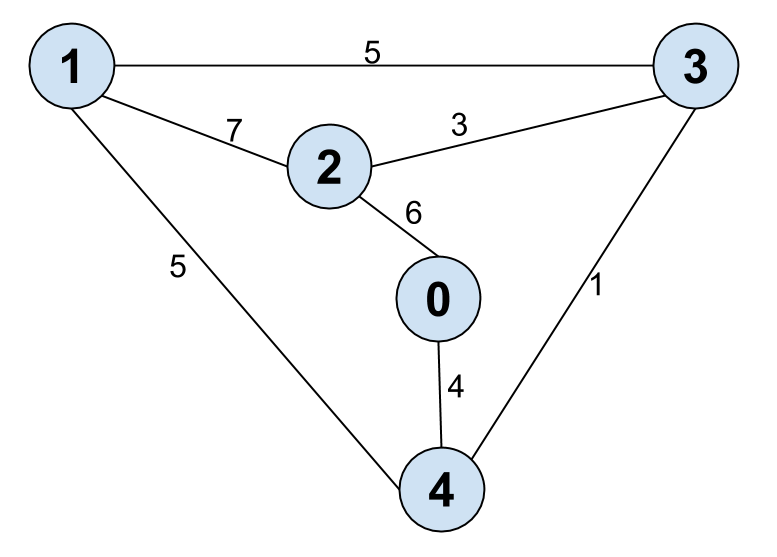
\includegraphics[scale=0.2]{Grafo_02}%
\begin{tabular}{|c|c|c|c|c|c|}
\hline 
I\textbackslash{}J & 0 & 1 & 2 & 3 & 4\tabularnewline
\hline 
\hline 
0 & 0 & 0 & 6 & 0 & 4\tabularnewline
\hline 
1 & 0 & 0 & 7 & 5 & 5\tabularnewline
\hline 
2 & 6 & 7 & 0 & 3 & 0\tabularnewline
\hline 
3 & 0 & 5 & 3 & 0 & 1\tabularnewline
\hline 
4 & 4 & 5 & 0 & 1 & 0\tabularnewline
\hline 
\end{tabular}\end{center}

\begin{center}

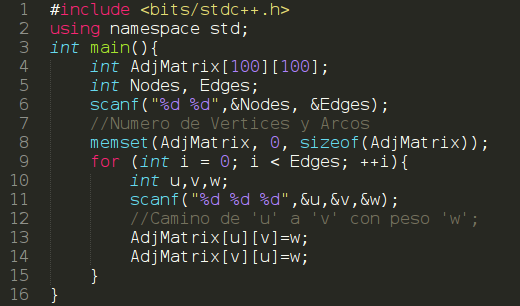
\includegraphics[scale=0.4]{Codigo_Grafo_02}

\end{center}


\subsection{Lista de Adyacencia}

Esta es la forma mas usual de representación de un grafo, la detallamos
a continuación:

\begin{center}

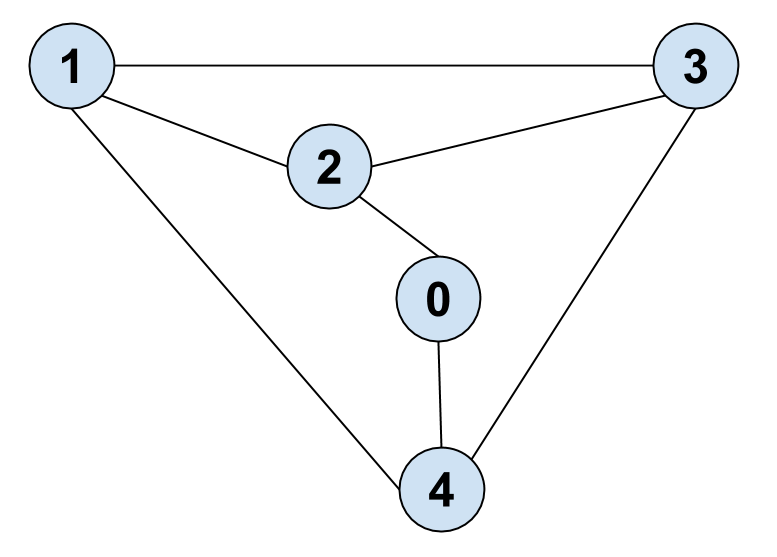
\includegraphics[scale=0.3]{Grafo_01}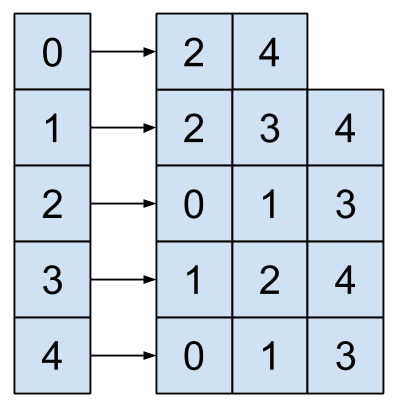
\includegraphics[scale=0.2]{AdjList_01}

\end{center}

Para representarlo en forma de Lista de Adyacencia usamos un vector
de vectores de enteros, en el cual la pocision 'i' tiene un vector
con todos los nodos que tengan un arco hacia 'i'. El codigo en C++
es el siguiente:

\begin{center}

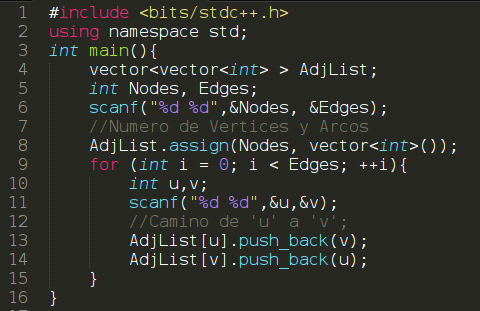
\includegraphics[scale=0.4]{Codigo_Grafo_03}

\end{center}

En el caso de un grafo ponderado usaremos un un vector de vectores
igual que antes, solo que ahora en lugar de guardar un entero guardaremos
un par de enteros con el peso y el nodo:

\begin{center}

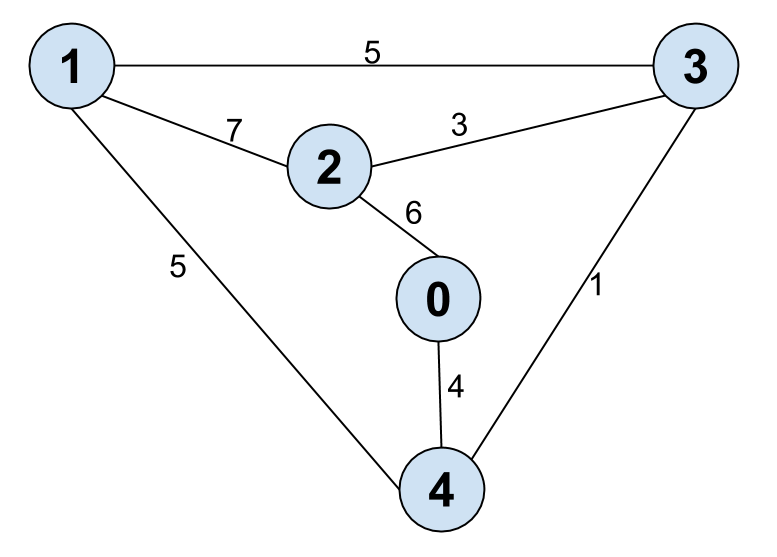
\includegraphics[scale=0.3]{Grafo_02} 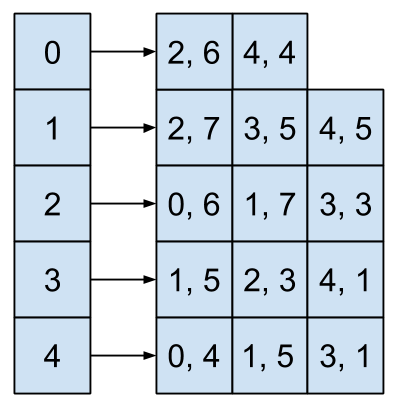
\includegraphics[scale=0.2]{AdjList_02}

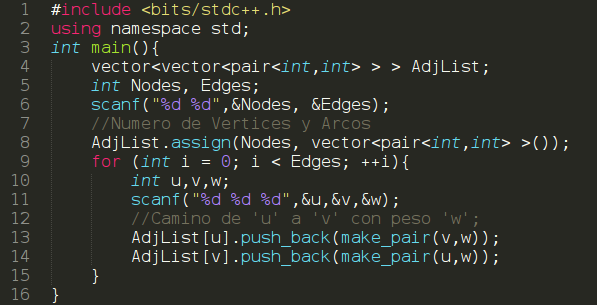
\includegraphics[scale=0.4]{Codigo_Grafo_04}

\end{center}


\section{Recorrido de un Grafo}

Una ves armado el grafo, viene lo realmente importante que es que
hacer con el en este caso lo que haremos seran 2 recorridos simples
en todo el grafo, estos son:


\subsection{BFS (Breadth First Search)}

Este algoritmo recorre el grafo de manera progresiva y ordenada, lo
recorre por niveles. BFS hace uso de una ``cola'' (queue) en la
que coloca los nodos que visitara, de esta manera al terminar de visitar
a los vecinos de la raíz continuara con los vecinos de estos y así
sucesivamente.

Ejemplo 2. Usaremos BFS para explorar el siguiente grafo:

\begin{center}

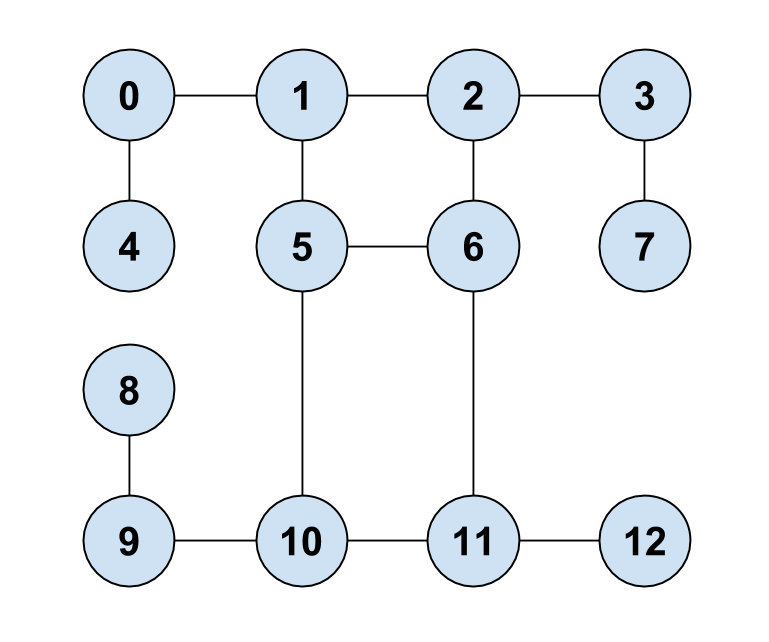
\includegraphics[scale=0.4]{BFS_01}

\end{center}

Tendremos como vértice raíz a 5,desde este nos expandiremos a todos
sus vecinos, comenzamos metiendo al 5 en la cola:

\begin{center}

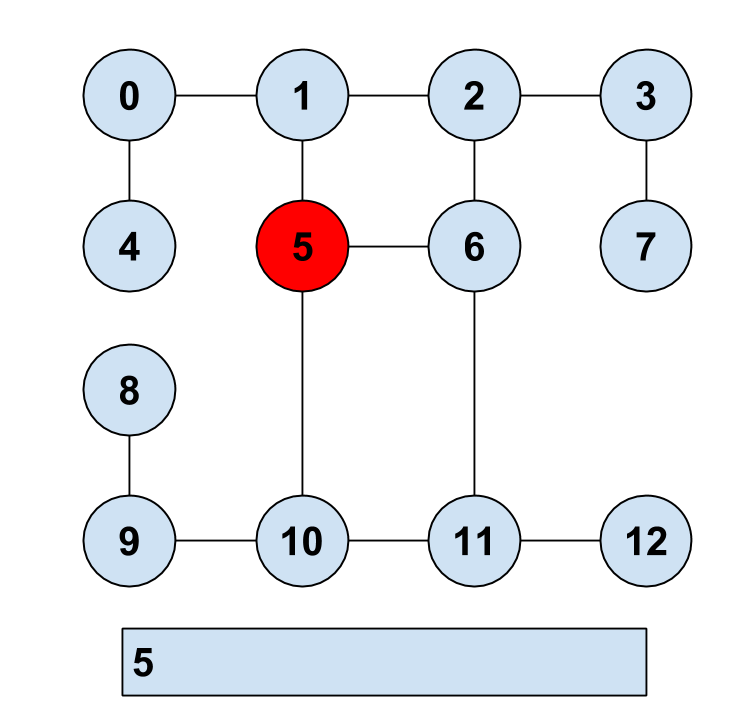
\includegraphics[scale=0.4]{BFS_02}

\end{center}

Ahora el algoritmo seguira corriendo mientras tengo vertices en la
cola, es decir mientras haya vertices por visitar, ahora que nos encontramos
en el vertice 5, lo sacamos de la cola y lo marcamos como visitado,
metemos a todos sus vecinos a la cola:

\begin{center}

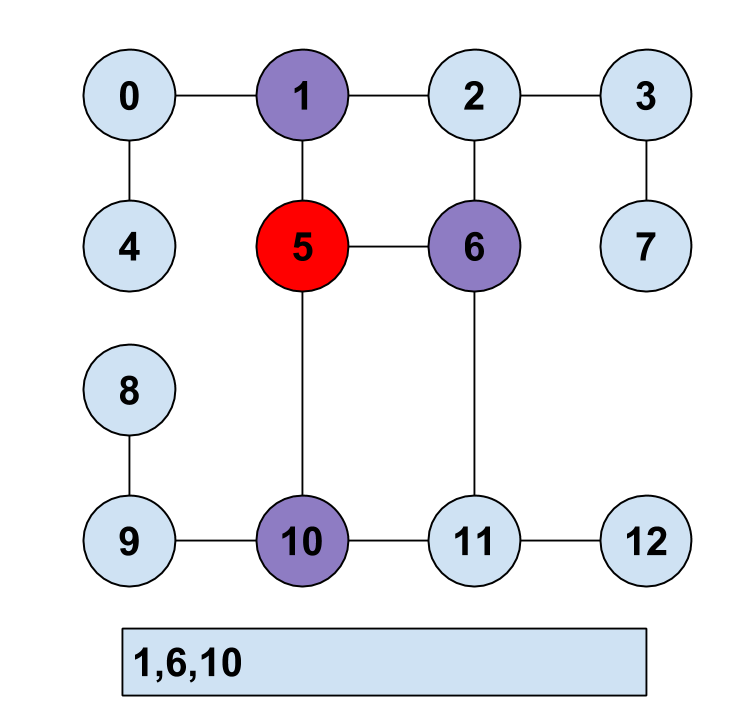
\includegraphics[scale=0.4]{BFS_03}

\end{center}

Ahora que estan todos sus vecinos en la cola, proseguimos con los
siguientes, el primero en la cola es el vértice 1, por lo cual lo
tomamos y encolamos a todos sus vecinos:

\begin{center}

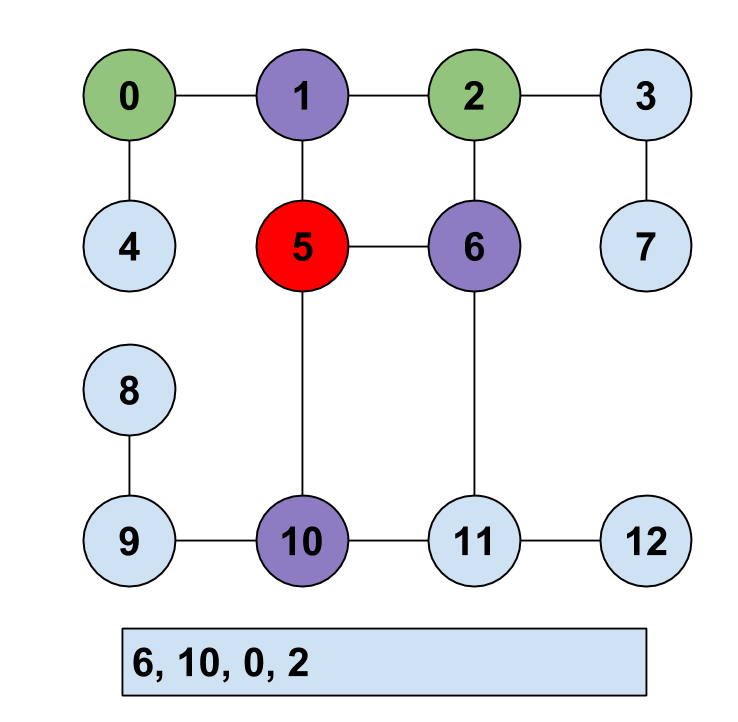
\includegraphics[scale=0.4]{BFS_04}

\end{center}

Ahora vamos viendo como funciona el algoritmo, toma el primer elemento
de la cola, lo visita, lo saca y encola a todos los vecinos de este,
es por esto que se da la exploración en forma de niveles, sigamos:

\begin{center}

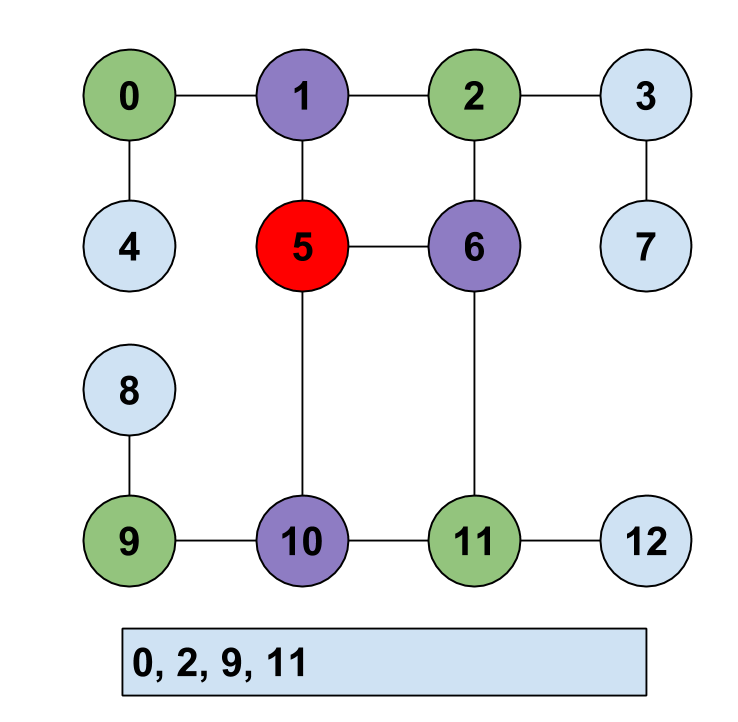
\includegraphics[scale=0.4]{BFS_05}

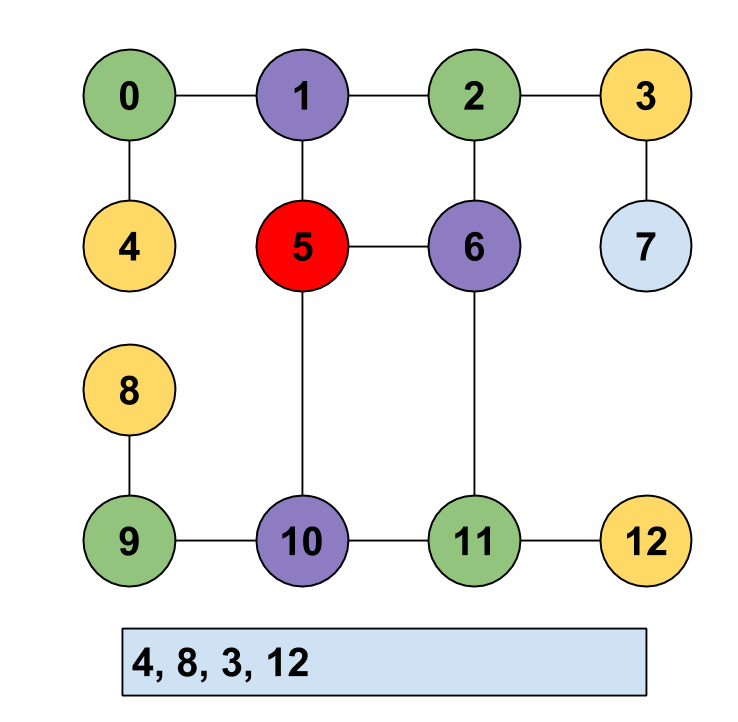
\includegraphics[scale=0.4]{BFS_06}

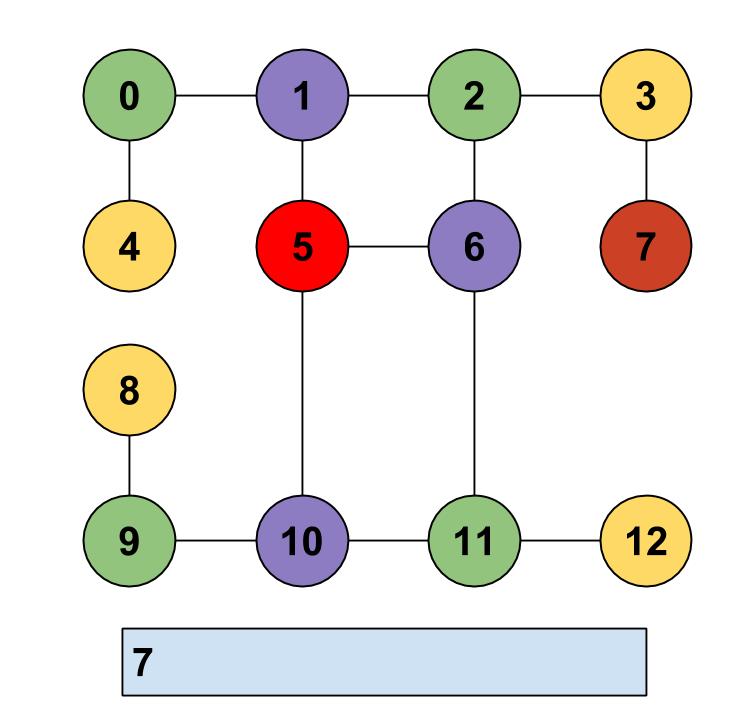
\includegraphics[scale=0.4]{BFS_07}

\end{center}

Ahora el ultimo elemento en la cola es 7 y como este no tiene vecinos
sin visitar, lo sacamos de la cola esta queda vacia y termina el algoritmo:

\begin{center}

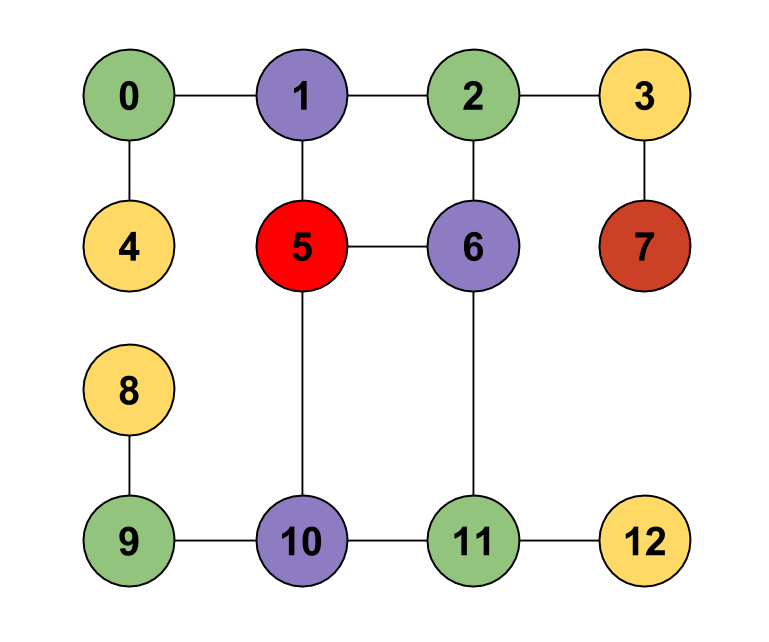
\includegraphics[scale=0.4]{BFS_08}

\end{center}

Como podemos ver BFS recorre todo el grafo y va formando niveles desde
la raiz.

Este es el codigo en C++ del BFS:

\begin{center}

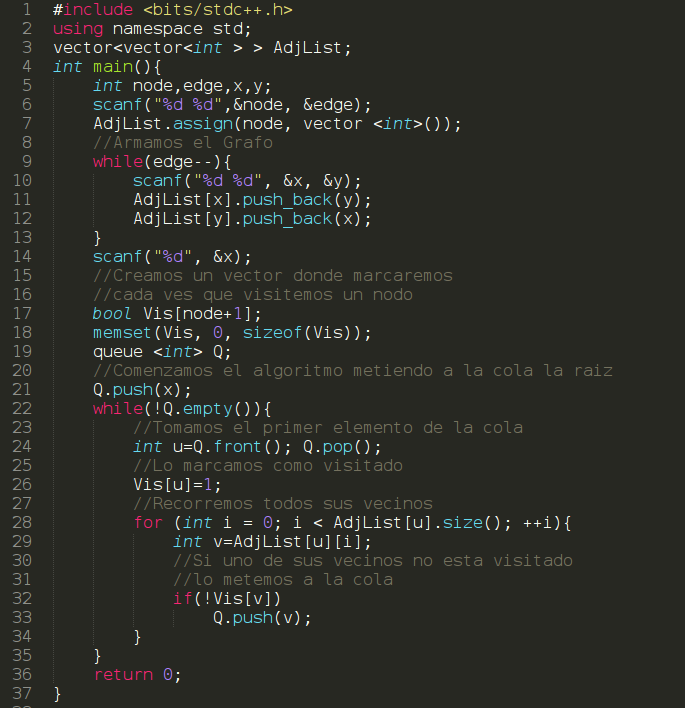
\includegraphics[scale=0.4]{Codigo_BFS}

\end{center}
\end{document}
